\chapter{Memoria di massa}
\section{Disco Rigido}
\subsection{Struttura}
\dfn{Hard Disk (HD)}{Un HD è composto da una serie di piatti o “dischi” sovrapposti, con un diametro che varia tra i 4,5 e i 9 cm.}

\begin{itemize}
    \item Ogni piatto è suddiviso in una serie di tracce circolari concentriche.
    \item Ogni traccia è suddivisa in una serie di settori.
    \item L’insieme delle tracce posizionate nello stesso punto sui vari piatti prende il nome di \textit{cilindro}.
    \item Un “braccio del disco” sostiene una testina di lettura/scrittura per ogni piatto: le testine si muovono tutte simultaneamente e si posizionano sui vari settori del piatto corrispondente (simile al braccio di un giradischi).
\end{itemize}

\nt{
    I settori del disco rappresentano l’unità minima di memorizzazione delle informazioni. Storicamente, ogni settore aveva una dimensione standard di 512 byte; tuttavia, dal 2010 molti produttori hanno aumentato la dimensione fino a 4 KB per settore. Ogni settore memorizza un blocco di dati.
}

\begin{itemize}
    \item I piatti dell'HD ruotano sincronicamente attorno al loro asse, raggiungendo velocità tra 5400 e 15000 RPM (\textit{rounds per minute}), corrispondenti a circa 250 giri al secondo.
    \item Ogni piatto ha associata una testina di lettura/scrittura dei settori, che opera a pochi micron dalla superficie del piatto.
\end{itemize}

\qs{Perché il tempo di accesso a un settore varia?}{
    Una testina può leggere o scrivere su un settore solo quando questo si trova esattamente sotto la testina. Pertanto, il tempo di accesso a un settore dipende principalmente da due componenti:
    \begin{itemize}
        \item \textit{Seek time} (tempo di posizionamento): il tempo necessario affinché la testina raggiunga la traccia contenente il settore desiderato.
        \item \textit{Rotational latency} (latenza rotazionale): il tempo che occorre affinché la rotazione del piatto allinei il settore esatto sotto la testina.
    \end{itemize}
}

\nt{
    A causa della presenza di elementi meccanici, i tempi di accesso sono dell’ordine di alcuni millisecondi.
}

\subsection{Mappatura degli indirizzi}
\dfn{Modello Logico di HD}{
    Un HD può essere logicamente visto come un array unidimensionale di blocchi logici, ciascuno di 512 (o più recentemente 4096) byte: questa è la più piccola unità di trasferimento dati.
}

\begin{itemize}
    \item Ogni settore corrisponde a un blocco logico.
    \item L’array unidimensionale di blocchi logici viene mappato sequenzialmente nei settori del disco:
    \begin{itemize}
        \item Il \textit{settore 0} è il primo settore della traccia più esterna del primo piatto (solitamente in posizione superiore o inferiore nella pila dei piatti).
        \item Successivamente, i settori vengono numerati consecutivamente lungo la traccia fino a raggiungere i settori delle tracce più interne. La numerazione prosegue in modo analogo nei restanti piatti.
    \end{itemize}
\end{itemize}

La mappatura tra blocco logico e settore del disco risulta più complessa di quanto sembri, a causa di due fattori principali:

\begin{itemize}
    \item \textbf{Difetti di fabbricazione:} I dischi possono avere settori difettosi. Tali settori vengono nascosti attraverso il meccanismo di mappatura, che associa blocchi logici a settori funzionanti del disco.
    \item \textbf{Differenze di lunghezza delle tracce:} Non tutte le tracce hanno la stessa lunghezza. 
    \begin{itemize}
        \item Le tracce più lontane dal centro del disco sono più lunghe rispetto a quelle interne e possono contenere fino al 40\% di settori in più.
    \end{itemize}
\end{itemize}

\subsection{Scheduling dei dischi rigidi}

Il sistema operativo (SO) riceve frequentemente richieste di accesso al disco da parte dei processi e deve ottimizzare il trasferimento dei dati per migliorare le prestazioni complessive di accesso al disco.

\nt{
    Il SO non può influenzare la \textit{latenza rotazionale} del disco, che in media corrisponde a metà del tempo necessario per completare una rotazione. Tuttavia, può ridurre il \textit{seek time medio} complessivo ordinando in maniera strategica le richieste in coda, minimizzando così il movimento delle testine.
}

\subsubsection{Algoritmi di scheduling delle richieste I/O}

Esistono diversi algoritmi per gestire lo scheduling delle richieste di I/O del disco. Consideriamo come esempio la seguente sequenza di richieste di accesso, comprese tra la traccia 0 e la traccia 199:

\[
\{ 98, 183, 37, 122, 14, 124, 65, 67 \}
\]

\nt{
    Le tracce potrebbero trovarsi su piatti diversi, dato che tutti i piatti ruotano insieme e le testine si muovono simultaneamente. Tuttavia, per semplicità possiamo supporre l’esistenza di un unico piatto e che la testina sia inizialmente posizionata sulla traccia (o cilindro) numero 53.
}

\begin{figure}[h] \centering 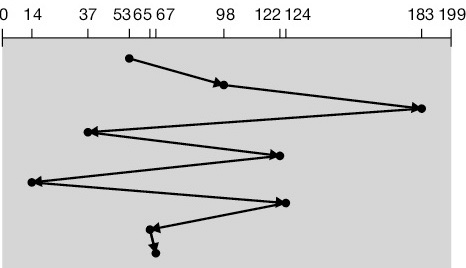
\includegraphics[width=0.25\linewidth]{images/scheduling_hdd_98.png}
\caption{Coda delle richieste: 98, 183, 37, 122, 14, 124, 65, 67 In tutto la testina attraversa 640 tracce. Invece che “122 - 14124” era meglio fare “122 - 124 - 14” }
\end{figure}

\subsubsection{C-SCAN (Circular-SCAN)}
Fornisce un tempo di attesa per le varie richieste più uniforme di altri algoritmi, anche se non riesce a garantire un tempo medio di attesa minimo.\\
La testina si muove da un estremo all’altro del piatto, servendo le richieste.\\
Quando raggiunge l’estremità del piatto, torna immediatamente all’inizio senza servire richieste.\\
In pratica, \textbf{tratta i settori/cilindri come una lista circolare.}\\

\begin{figure}[h] \centering 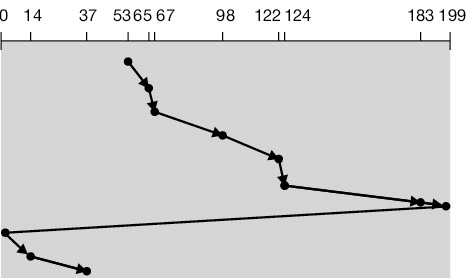
\includegraphics[width=0.25\linewidth]{Teoria/images/scheduling_hdd_cscan.png}
    \caption{Coda delle richieste: 98, 183, 37, 122, 14, 124, 65, 67 La testina attraversa 183 tracce + 200 tracce per tornare indietro, ma questo ritorno richiede poco tempo, perché la
    testina non deve mai fermarsi e ripartire}
\end{figure}

\nt{Questo è l'algoritmo di scheduling più utilizzato nei sistemi operativi moderni.}


\section{Formattazione del disco}
Prima di poter essere utilizzato, un disco rigido deve essere sottoposto a un processo di \textit{formattazione}, che avviene in due fasi principali:

\begin{itemize}
    \item Questa operazione viene solitamente effettuata dal costruttore dell’HD e ha lo scopo di:
    \begin{itemize}
        \item Associare un numero univoco a ogni settore.
        \item Allocare uno spazio per un codice di correzione degli errori (ECC), utilizzato durante ogni operazione di I/O su quel settore.
    \end{itemize}
    \item Durante questa fase è possibile definire la dimensione dei blocchi fisici, ad esempio 512 byte o 4096 byte per settore.
\end{itemize}

\subsubsection{Formattazione logica}

\begin{itemize}
    \item Questo processo, gestito dal sistema operativo, è necessario per creare e organizzare il File System.
    \item Il sistema operativo esegue le seguenti operazioni:
    \begin{itemize}
        \item Creazione della lista dei blocchi liberi secondo lo schema adottato.
        \item Creazione di una directory iniziale, punto di partenza per l’intera struttura del File System.
        \item Riservazione di aree specifiche per la gestione diretta da parte del SO:
        \begin{itemize}
            \item \textbf{Boot Block:} il blocco di avviamento.
            \item \textbf{Aree per gli attributi dei file:} ad esempio, gli \textit{index-node} in Unix o la MFT (\textit{Master File Table}) in Windows.
        \end{itemize}
    \end{itemize}
\end{itemize}

\subsection{Il Boot Block}

\begin{itemize}
    \item Contiene il codice necessario per avviare il sistema operativo.
    \item All’accensione, un piccolo programma residente in ROM istruisce il \textit{disk controller} a trasferire il contenuto del Boot Block nella RAM.
    \item Una volta trasferito, il controllo passa al codice del Boot Block, che avvia l’intero sistema operativo caricandolo dal disco stesso.
\end{itemize}

\section{Gestione dell'area di SWAP}
Durante la formattazione logica del disco rigido, il sistema operativo riserva uno spazio per l'\textit{area di Swap}, che funge da memoria virtuale utilizzata per lo scambio di pagine o segmenti tra RAM e memoria secondaria.

\subsection{Gestione dell'area di Swap}

\begin{itemize}
    \item \textbf{Swap come file:} 
    \begin{itemize}
        \item Nel caso più semplice, l’area di Swap può essere un file di grandi dimensioni all’interno del File System.
        \item Nei sistemi Windows, lo \textit{swap file} è denominato \texttt{pagefile.sys}. 
        \item Gli utenti possono regolarne la dimensione, ad esempio riducendola in presenza di una grande quantità di RAM, per recuperare spazio sul disco rigido.
    \end{itemize}

    \item \textbf{Swap come partizione dedicata:}
    \begin{itemize}
        \item Una porzione specifica del disco rigido, chiamata \textit{partizione di Swap}, può essere riservata esclusivamente a questo scopo.
        \item Questa partizione è gestita diversamente rispetto a un normale File System, adottando strategie di allocazione ottimizzate per la velocità di accesso.
        \item Ad esempio, i blocchi possono essere allocati in modo contiguo per evitare la ricerca di blocchi liberi, riducendo così il tempo necessario per lo scambio.
    \end{itemize}
\end{itemize}

\subsubsection{Dimensionamento dell'area di Swap}

\nt{
    È fondamentale dimensionare adeguatamente l’area di Swap per garantire che il sistema operativo trovi rapidamente uno spazio libero per lo scambio di pagine e segmenti.
}

\begin{itemize}
    \item \textbf{Consigli per il dimensionamento:}
    \begin{itemize}
        \item In Solaris, si raccomanda di dimensionare l’area di Swap in base alla differenza tra lo spazio di indirizzamento logico e quello fisico.
        \item In Linux, si suggerisce di utilizzare un’area di Swap pari al doppio della RAM disponibile.
    \end{itemize}
    
    \item \textbf{Sistemi con più dischi:}
    \begin{itemize}
        \item In configurazioni multi-disco, è possibile creare un’area di Swap per ciascun disco.
        \item Ciò consente di sfruttare le aree di Swap in parallelo, bilanciando il carico di lavoro e migliorando le prestazioni.
    \end{itemize}
\end{itemize}


\section{Sistemi RAID}
Gli hard disk (HD) e i dischi a stato solido (SSD) sono dispositivi notevolmente più lenti rispetto al processore e alla memoria primaria. Inoltre, il guasto di un disco rigido rappresenta un rischio significativo: in assenza di un back-up, i dati memorizzati possono essere irrimediabilmente persi o, nel migliore dei casi, non disponibili durante i tempi di riparazione.

\subsection{Introduzione ai sistemi RAID}

\dfn{RAID (Redundant Array of Independent Disks)}{
    È un sistema di configurazione della memoria secondaria progettato per migliorare sia le prestazioni sia l'affidabilità degli hard disk. 
}

\begin{itemize}
    \item RAID si rivela utile in ogni settore, ma è essenziale in contesti critici dove il servizio non può mai interrompersi, come nel settore finanziario e bancario.
    \item Il concetto di RAID fu introdotto nel 1988 da Patterson, Gibson e Katz, con l'acronimo iniziale \textit{Redundant Array of Inexpensive Disks}, successivamente ridefinito come \textit{Redundant Array of Independent Disks}.
    \item La controparte dei sistemi RAID è rappresentata da dispositivi SLED (\textit{Single Large Expensive Disk}).
\end{itemize}

\subsection{Caratteristiche principali di un sistema RAID}

\begin{itemize}
    \item Un sistema RAID è costituito da un insieme di dischi (detto \textit{disk array}) che viene visto dal sistema operativo come un singolo dispositivo di memorizzazione, più veloce e affidabile di un SLED.
    \item La gestione dei dischi è demandata al \textit{controller del RAID}, che si occupa di distribuire i dati secondo criteri specifici, senza necessità di modifiche al sistema operativo. 
    \item Questo vantaggio semplifica notevolmente la vita degli amministratori di sistema (\textit{system administrators}).
\end{itemize}

\subsection{Idee principali alla base di RAID}

Le due idee fondamentali di un sistema RAID sono:
\begin{enumerate}
    \item \textbf{Distribuzione dei dati:} L'informazione è suddivisa su più dischi per parallelizzare parte delle operazioni di accesso e migliorare le prestazioni.
    \item \textbf{Ridondanza dei dati:} L'informazione è duplicata su più dischi. In caso di guasto di un disco, il sistema può continuare a funzionare, recuperando i dati dal disco di backup.
\end{enumerate}

\subsection{Livelli di RAID}

Differenti schemi di implementazione delle idee sopra descritte hanno portato alla definizione di vari livelli RAID, numerati da 0 a 6. 
\nt{
    Da qui in poi, ci si discosta parzialmente dalla trattazione del libro di testo.
}
\subsection{RAID di Livello 0}

\nt{
    I sistemi RAID di livello 0, pur essendo inclusi nella famiglia RAID, non offrono ridondanza dei dati, quindi non aumentano l'affidabilità del sistema.
}

\dfn{RAID Livello 0}{
    Un'architettura RAID in cui il disco virtuale (cioè l'insieme di blocchi logici consecutivi visti dal sistema operativo) viene suddiviso in \textit{strip} (strisce) di $k$ blocchi consecutivi ciascuna. Questa tecnica, chiamata \textbf{striping}, distribuisce i dati su più dischi per migliorare le prestazioni.
}

\begin{itemize}
    \item Ogni \textit{strip} è identificata da un numero e contiene $k$ blocchi consecutivi.
    \begin{itemize}
        \item Lo strip 0 contiene i blocchi da $0$ a $k-1$.
        \item Lo strip 1 contiene i blocchi da $k$ a $2k-1$.
    \end{itemize}
    \item Gli strip sono distribuiti sui dischi disponibili secondo la formula:
    \[
    \text{numero-strip} \mod \text{dischi-nel-sistema}
    \]
    \item Ad esempio, in un sistema con 4 dischi:
    \begin{itemize}
        \item Il disco 0 conterrà gli strip 0, 4, 8, ...
        \item Il disco 1 conterrà gli strip 1, 5, 9, ...
    \end{itemize}
    \item Se $k=1$, ogni strip contiene un singolo blocco. In questo caso:
    \begin{itemize}
        \item Il blocco 0 sarà sul primo settore del primo disco.
        \item Il blocco 1 sarà sul primo settore del secondo disco.
        \item Il blocco 4 sarà sul secondo settore del primo disco, e così via.
    \end{itemize}
\end{itemize}

\ex{Esempio di richiesta su un RAID Livello 0}{
    Supponiamo che il sistema operativo richieda la lettura di dati contenuti negli strip 4, 5, 6 e 7. 
    \begin{itemize}
        \item Il controller RAID suddividerà la richiesta in quattro letture parallele, una per ciascun disco.
        \item Su un singolo disco SLED, invece, tutti i settori dei quattro strip dovrebbero essere letti in sequenza.
    \end{itemize}
    Di conseguenza, l'operazione sarà completata più rapidamente con il RAID 0.
}

\clm{Prestazioni e limiti del RAID Livello 0}{}{
    \begin{itemize}
        \item \textbf{Miglioramenti delle prestazioni:} Un RAID di livello 0 è particolarmente efficiente quando le richieste coinvolgono molti strip consecutivi, e il sistema è composto da un elevato numero di dischi.
        \item \textbf{Limitazioni:}
        \begin{itemize}
            \item Richieste che riguardano un singolo strip non ottengono alcun miglioramento rispetto a un disco SLED.
            \item L'affidabilità del sistema è inferiore a quella di un singolo disco SLED, poiché il \textit{Mean Time To Failure} (MTTF) complessivo diminuisce con l'aumento del numero di dischi.
        \end{itemize}
        \item \textbf{Applicazioni tipiche:} Il RAID 0 è utilizzato in applicazioni che richiedono alte prestazioni ma non necessitano di particolare affidabilità, come lo streaming audio e video.
    \end{itemize}
}
\begin{figure}[h] \centering 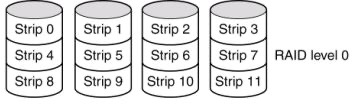
\includegraphics[width=0.50\linewidth]{images/raid_livelloZero.png} \caption{Raid Livello Zero} \label{fig:2-23a} \end{figure}
